%\iffalse
%\section{Introduction to Automated Theorem Proving}
%Automated Theorem Proving (ATP) is a critical area within automated reasoning that focuses on the development of computer programs capable of proving mathematical theorems automatically. ATP systems are designed to assist mathematicians, logicians, and computer scientists in validating the correctness of propositions and theorems without human intervention.
%
%\section{The Boolean Satisfiability Problem}
%\begin{tcolorbox}[colframe=defcolor,title={\color{white}\bf Propositional Variable}]
%\begin{definition}
%A \textbf{propositional variable} is an input variable (that can either be true or false) of a truth function. Propositional variables are the \textit{basic building-blocks} of propositional formulas, used in propositional logic and higher-order logics.
%\end{definition}
%\end{tcolorbox}
%\begin{example}
%For a statement variable, a lowercase letter is usually used, for example:
%$p,q,r,\dots$, and so on
%or lowercase Greek letters, for example:
%$\phi, \psi, \chi$ and so on.
%\end{example}
%\begin{remark}
%The citing of a propositional variable can be interpreted as an assertion that the proposition represented by that symbol is true.
%That is:
%\begin{quote}
%"$p$" means "$p$ is true".
%\end{quote}
%\end{remark}
%
%\begin{tcolorbox}[colframe=defcolor,title={\color{white}\bf Propositional Function (Formula)}]
%\begin{definition}
%A \textbf{propositional function} (or \textbf{formula}) $P(x_1,x_2,\dots)$
%is an operation which acts on the objects denoted by the object variables (here, propositional variables) $x_1,x_2,\dots$
%in a particular universe to return a truth value which depends on:
%\begin{enumerate}[(1)]
%	\item The values of $x_1,x_2,\dots$
%	\item The nature of $P$.
%\end{enumerate}
%\end{definition}
%\end{tcolorbox}
%
%The boolean satisfiability problem (SAT) is the following: given a formula $F$ on propositional variables, does there exists an assignment $\mathcal{A}$ on theses variables, such that $\mathcal{A}(F)=1$.
%
%Given a formula $F$ over a set of propositional variables $\set{x_1,x_2,\dots,x_n}$, \[
%\exists\mathcal{A}:\set{x_1,x_2,\dots,x_n}\to\set{0,1}:\mathcal{A}(F)=1.
%\]
%\newpage
%\fi

\section{The Boolean Satisfiability Problem}
\begin{tcolorbox}[colframe=defcolor,title={\color{white}\bf Propositional Function (Formula)}]
\begin{definition}
A \textbf{propositional function} (or \textbf{formula}) is defined inductively as follows:
\begin{itemize}
	\item[] (Basic Step) Any propositional variable $x\in V$ is a formula.
	\item[] (Inductive Step) If $F$ and $G$ are formulas, then the following are also formulas:
	\begin{itemize}
		\item $\lnot F$
		\item $F\land G$
		\item $F\lor G$
		\item $F\rightarrow G$
		\item $F\leftarrow G$
	\end{itemize}
\end{itemize}
Formally, the set of all $\Phi$ is the smallest set satisfying: \[
\Phi = V\cup\set{\lnot F:F\in\Phi}\cup\set{\circ(F,G):F,G\in\Phi\ \text{and}\ \circ\in\set{\land,\lor,\rightarrow,\leftrightarrow}}
\]
\end{definition}
\end{tcolorbox}

\begin{tcolorbox}[colframe=defcolor,title={\color{white}\bf Boolean Satisfiability Problem (SAT)}]
\begin{definition}
Let $X=\set{x_1,x_2,\cdots, x_n}$ be a set of propositional variables.

Let $L$ be a set of one or more propositional formulas constructed using only:
\begin{itemize}
	\item $x_i\in X$ for $i=1,\dots,n$;
	\item the $2^{(2^1)}=4$ unary logical connectives;
	\item the $2^{(2^2)}=16$ binary logical connectives;
\end{itemize}
The problem is to find truth values for all $x\in X$
such that all the formulas in $L$ are true.

Such a problem is a boolean satisfiability problem.
\end{definition}
\end{tcolorbox}

\newpage

\begin{note}[literal]
A \textit{literal} is either a propositional variable ($p$) or its negation ($\lnot p$).
\end{note}

\begin{tcolorbox}[colframe=defcolor,title={\color{white}\bf Conjunctive Normal Form (CNF)}]
\begin{definition}
A formula $F$ is in conjunctive normal form (CNF) if and only if it is a conjunction of disjunctions of literals, i.e. of the form \[
F=\bigvee_i\bigwedge_jl_{i,j}
\] where $l_{i,j}$ are the literals.
\end{definition}
\end{tcolorbox}
\begin{remark}
Usually, CNF formulae are represented in an alternative form called
clauses using the commutativity, associativity and idempotence of the logical
operators $\lor$ and $\land$. A clause corresponds to a disjunction of literals and a CNF
formula is a conjunction of clauses. We write a clause as a set of its literals and
a formula as a set of clauses. 
\end{remark}

\begin{example}
\ \begin{table}[h!]\centering\setstretch{1.5}
\begin{tabular}{rl}
	A propositional formula: & $\lnot(((x_0\land\lnot x_1)\lor x_2)\leftrightarrow x_1)$ \\
	An equivalent formula in CNF: & $(x_0\lor x_1\lor x_2)\land (\lnot x_1\lor \lnot x_2)$ \\
	In clause representation: & $\set{\set{x_0,x_1,x_2},\set{\lnot x_1,\lnot x_2}}$
\end{tabular}
\end{table}\\
In reality, formulae are often not being transformed into equivalent CNF formulae but into equisatisfiable CNF formulae (formulae which are satisfiable if
and only if the original formula is satisfiable) when preparing them for SAT,
because this can be done efficiently.
\end{example}

\newpage
\section{Basics of SAT Solving}

The Conflict Driven Clause Learning (CDCL) algorithm is a mix of two older approaches to SAT solving: Davis–Putnam–Logemann–Loveland (DPLL) and Resolution. It uses concepts from both and combines them in a new way.

\subsection{Backtracking and Unit Propagation as in DPLL Solvers}
\begin{example}
Example graph for $G=\set{\set{\lnot x_0,\lnot x_1,\lnot x_2},\set{\lnot x_0,x_2},\set{x_0,x_1,x_2}}:$
\begin{center}
	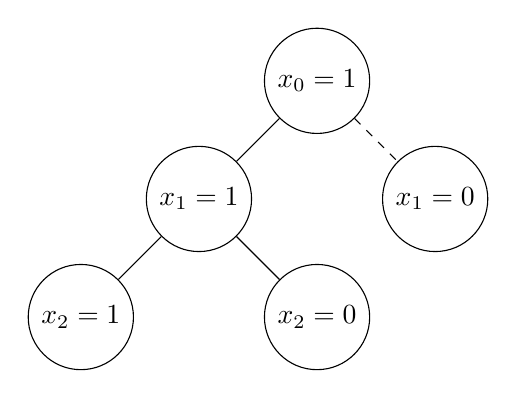
\begin{tikzpicture}
		[level distance=15mm,
		every node/.style={circle,draw},
		level 1/.style={sibling distance=30mm},
		level 2/.style={sibling distance=30mm}]
		\node {$x_0 = 1$}
		child {node {$x_1 = 1$}
			child {node {$x_2 = 1$}}
			child {node {$x_2 = 0$}}}
		child {node {$x_1 = 0$}
			edge from parent[dashed]};
	\end{tikzpicture}
\end{center}
The backtracking algorithm has just discovered that setting $x_2 = 0$ makes the
clause $\set{\lnot x_0 , x_2}$ false. So it goes back to explore the $x_1 = 0$ path and deletes
the value of $x_2$.
\end{example}
\subsection{Resolution}

If a formula \(F\) contains the clauses \(\{\neg x\} \cup A\) and \(\{x\} \cup A\)...

\newpage
\section{Principles of CDCL}

Now that we have seen how Backtracking and Resolution work we are ready to merge these approaches...

\subsection{The trail}

When applying CDCL rather than exploring a search tree of assignments...

\subsection{Conflict clauses and backjumping}

Consider our previous example again. When we want to continue building up our trail...

\subsection{The implication graph}

A nice way to illustrate the functionality of CDCL are implication graphs...

\subsection{The algorithm}

To get a clearer view Algorithm 4.1 shows the pseudocode for the CDCL algorithm...

\section{Implementation}

Let us now look at how the algorithm is implemented in real life...

\subsection{Clauses}

We use a monolithic array MEM to hold the original formula’s clauses as well as the newly learned clauses...

\subsection{Literals}

Assume the variables are \(x_1, x_2, \ldots, x_n\). We represent \(x_k\) by \(k\)...

\section{Results}

It is important to say that CDCL is a sound and complete algorithm for the propositional satisfiability problem...
